% L11c lecture companion. Notebook hashes and coverage are recorded in README.md.
% Style files and Cornell seal are copied unchanged from the L10c deck (identical
% to L10a, L9c, and L9a, which match the approved L6a deck). The grid world
% figure is converted from the notebook SVG in ../figs by `make figures`.
%
% Notation follows the lecture: the MDP tuple (S, A, R(s,a), T(s'|s,a), gamma),
% available actions A_s, observed rewards r, the policy pi, value functions U_k,
% U^*, action values Q_1(s,a), the tolerance epsilon, the iteration limit k_max,
% and for random rollout the depth d, number of rollouts N, return G, visit
% counts n(s), the estimate \hat{U}(s), and the bound r_max.
\documentclass[aspectratio=169,11pt]{beamer}
\usepackage{vnslides}
\renewcommand{\vnlecturecode}{L11c}
\newcommand{\lecturelink}{https://github.com/varnerlab/CHEME-5800-CourseRepository-Fall-2026/blob/main/weeks/week-11/L11c/CHEME-5800-L11c-Lecture-MarkovDecisionProcesses-Fall-2026.ipynb}
\newcommand{\examplelink}{https://github.com/varnerlab/CHEME-5800-CourseRepository-Fall-2026/blob/main/weeks/week-11/L11c/CHEME-5800-L11c-Example-RandomRollout-Fall-2026.ipynb}
\newcommand{\lablink}{https://github.com/varnerlab/CHEME-5800-CourseRepository-Fall-2026/blob/main/weeks/week-11/L11d/CHEME-5800-L11d-Lab-ValueIterationGridWorld-Fall-2026.ipynb}
\newcommand{\lecturesource}[1]{\note{[Sources]\par
  \href{\lecturelink}{L11c lecture: Markov Decision Processes (MDPs).}\par
  #1\par[/Sources]}}
\newcommand{\Sset}{\mathcal S}
\newcommand{\Aset}{\mathcal A}
\newcommand{\Uh}{\hat{U}}

\title{\texorpdfstring{{\vnheavy L11c}}{L11c}: Markov Decision Processes}
\subtitle{\texorpdfstring{Value iteration and random rollout\\[3pt]CHEME 5800 Cornell University}{Value iteration and random rollout; CHEME 5800 Cornell University}}
\author{Copyright Jeffrey Varner 2026. All Rights Reserved}

\begin{document}
\special{pdf:minorversion 7}
\vntitlepage

\begin{frame}{Objectives for Today}
  How should an agent choose its actions when each action changes both the
  reward it collects and the state it moves to?

  \vspace{0.4em}
  {\large\textbf{\ink{Today's concepts}}}
  \vspace{0.2em}
  \begin{itemize}\setlength{\itemsep}{0.4em}
    \item \hilite{Formulate a Markov decision process}: define its states,
      actions, rewards, transition model, and discount factor, and the policy
      that chooses an action in each state.
    \item \hilite{Solve for the optimal policy with value iteration}: update the
      value of each state from the states it can reach next until the values
      stop changing.
    \item \hilite{Estimate values with random rollouts}: average the discounted
      rewards of simulated random trajectories, without writing down the
      transition probabilities.
  \end{itemize}
  \slidenote{Lecture:}{\href{\lecturelink}{Markov Decision Processes (MDPs)}}
  \lecturesource{Introduction and three Learning Objectives.}
\end{frame}

\begin{frame}{Lecture and Example}
  \textbf{\ink{Lecture:}}
  \href{\lecturelink}{Markov Decision Processes (MDPs)}

  In this lecture, we formulate Markov decision processes, solve them with
  value iteration, and estimate values with random rollouts.

  \vspace{1.1em}
  \textbf{\ink{Example:}}
  \href{\examplelink}{Value Iteration and Random Rollout in the Slippery Grid World}

  In this example, we solve the lecture's grid world with value iteration,
  estimate its values with random rollouts, and compare the two answers.

  \vspace{0.8em}
  A rollout needs only a simulator; value iteration needs the full transition
  model.
  \lecturesource{Introduction and Example.}
\end{frame}

\begin{frame}{From Markov Chains to Decisions}
  A Markov decision process (MDP) extends the Markov chain by adding
  \hilite{actions} and \hilite{rewards}.

  \vspace{0.6em}
  \begin{itemize}\setlength{\itemsep}{0.7em}
    \item A Markov chain evolves passively, according to fixed transition
      probabilities.
    \item In an MDP, an agent chooses actions that influence the state
      transitions and generate rewards.
  \end{itemize}

  \vspace{0.8em}
  MDPs are the foundation for sequential decision-making under uncertainty:
  the agent must make good decisions, one after another, in a stochastic
  environment.
  \lecturesource{Introduction: opening paragraph.}
\end{frame}

\begin{frame}{MDP Components}
  An MDP is defined by the tuple
  $\left(\Sset,\Aset,R(s,a),T(s'\,|\,s,a),\gamma\right)$:

  \vspace{0.3em}
  \begin{itemize}\setlength{\itemsep}{0.35em}
    \item \hilite{State space} $\Sset$: all possible states $s$ of the system.
    \item \hilite{Action space} $\Aset$: all possible actions $a$; the actions
      available in state $s$ are $\Aset_s\subseteq\Aset$.
    \item \hilite{Reward function} $R(s,a)$: the expected immediate reward of
      action $a$ in state $s$. One transition produces an observed reward $r$.
    \item \hilite{Transition model}
      $T(s'\,|\,s,a)=P(s_{t+1}=s'\,|\,s_t=s,a_t=a)$: the probability that
      action $a$ in state $s$ leads to state $s'$.
    \item \hilite{Discount factor} $\gamma\in[0,1)$: weights future rewards
      against immediate ones; $\gamma=0$ cares only about now, and $\gamma\to1$
      values long-term returns.
  \end{itemize}
  \lecturesource{MDP Components: the tuple and the five components.}
\end{frame}

\begin{frame}{Policies and Terminal States}
  The agent's goal is a \hilite{policy} $\pi:\Sset\to\Aset$, with $\pi(s)=a$,
  that maximizes the expected cumulative discounted reward:
  \[
    \mathbb E\left[\sum_{t=0}^{\infty}\gamma^{t}R(s_t,a_t)\right].
  \]
  {\small Previously, $\pi$ denoted a state distribution; here it is a policy.}

  \vspace{0.5em}
  In an episodic problem, entering a \hilite{terminal state} ends reward
  collection:
  \begin{itemize}\setlength{\itemsep}{0.3em}
    \item The reward for reaching the terminal state is collected on entry.
    \item Value iteration treats it as absorbing: a dummy action keeps the agent
      there and earns zero reward, so its value stays zero.
  \end{itemize}

  \vspace{0.3em}
  Today: \hilite{value iteration} solves for the optimal policy, and
  \hilite{random rollout} estimates the value of a state by simulation.
  \lecturesource{MDP Components: the goal, the terminal-state paragraph, and the two algorithms. The note on the symbol pi is added for the deck.}
\end{frame}

\begin{frame}{Example: Grid World Navigation}
  A robot navigates a $3\times3$ grid to reach a goal while avoiding an
  obstacle and minimizing travel time:

  \vspace{0.3em}
  \begin{itemize}\setlength{\itemsep}{0.3em}
    \item \hilite{States}: the eight squares $(x,y)$, $x,y\in\{1,2,3\}$, other
      than the obstacle at $(2,2)$; $x$ increases to the right and $y$ upward.
    \item \hilite{Actions}: up, down, left, right; moves off the grid are
      unavailable, so $\Aset_s\subsetneq\Aset$ on the edges.
    \item \hilite{Rewards}: $+10$ for entering the goal at $(3,3)$, $-5$ for a
      bump into the obstacle, and $-1$ for every other outcome, including a slip
      off the grid.
    \item \hilite{Transitions}: slippery terrain; the intended move succeeds with
      probability $0.8$, and each perpendicular move happens with probability
      $0.1$.
    \item \hilite{Discount factor} $\gamma=0.9$: the $+10$ goal outweighs the
      $-1$ step costs, so the robot pursues the goal.
  \end{itemize}
  \lecturesource{MDP Components: Example: Grid World Navigation, the five components.}
\end{frame}

\begin{frame}{Grid World: The Layout}
  \centering
  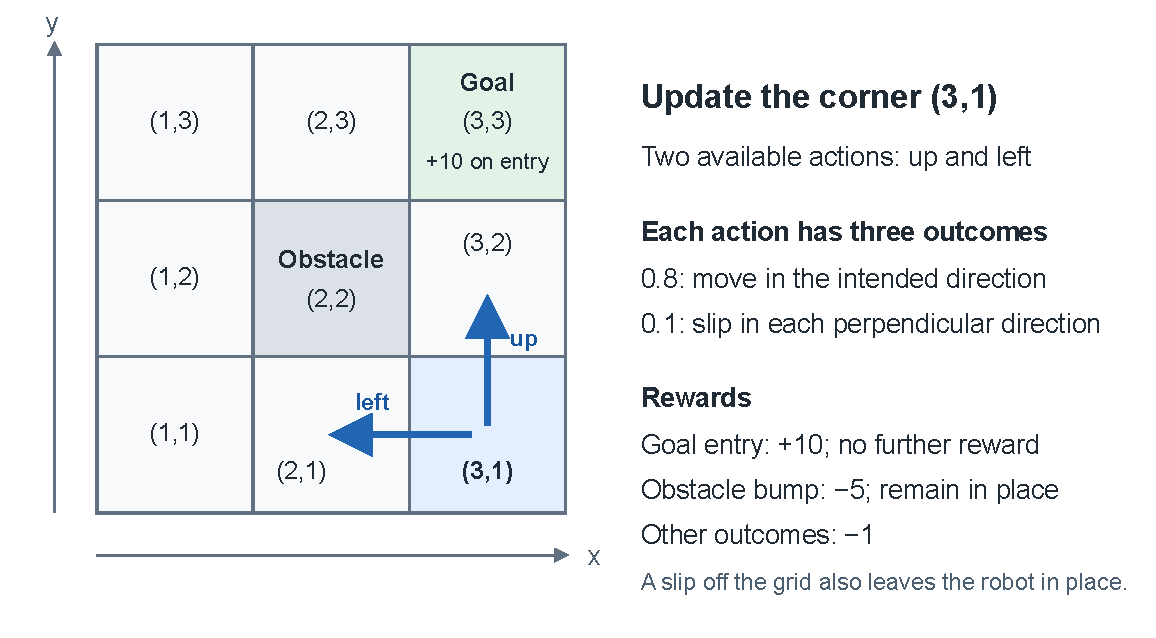
\includegraphics[width=\textwidth,height=0.64\paperheight,keepaspectratio]{assets/Fig-GridWorld-Backup.pdf}

  \vspace{0.3em}
  \raggedright
  Because moves are random, $R(s,a)$ averages over where the robot actually
  moves. A bump or a slip off the grid leaves it in place, and the goal is
  terminal.
  \lecturesource{MDP Components: the paragraph after the grid world components, the figure, and the closing sentence on pi^*.
    Figure: ../figs/Fig-GridWorld-Backup.svg (light colors).}
\end{frame}

\begin{frame}{Value Iteration}
  Value iteration is a \hilite{dynamic programming} algorithm: it builds the
  value of each state from the values of the states that can follow it. It
  repeats the \hilite{Bellman backup}:
  \[
    U_{k+1}(s)=\max_{a\in\Aset_s}\left(R(s,a)+\gamma\sum_{s'\in\Sset}T(s'\,|\,s,a)\,U_k(s')\right)
  \]

  \vspace{0.3em}
  \begin{itemize}\setlength{\itemsep}{0.5em}
    \item For $0\le\gamma<1$, $U_k(s)\to U^{*}(s)$ as $k\to\infty$.
    \item The \hilite{optimal value function} $U^{*}(s)$ is the maximum
      expected cumulative discounted reward achievable from state $s$ under the
      best possible policy.
  \end{itemize}
  \lecturesource{Value Iteration: definition, Bellman backup, and convergence paragraph.}
\end{frame}

\begin{frame}{Worked Example: One Bellman Backup}
  Update the corner $s=(3,1)$, whose available actions are up and left. Every
  outcome of either action earns $-1$.

  \vspace{0.3em}
  Starting from $U_0=0$, the first sweep gives:
  \[
    U_1(3,2)=7.4,\qquad U_1(2,1)=-1.4,\qquad U_1(3,1)=-1.
  \]

  \vspace{0.2em}
  For example, $7.4$ comes from moving up from $(3,2)$:
  \[
    0.8\,(+10)+0.1\,(-5)+0.1\,(-1)=7.4,
  \]
  reaching the goal with probability $0.8$, bumping the obstacle with
  probability $0.1$, and slipping off the grid with probability $0.1$.
  \lecturesource{Value Iteration: Example: One Bellman Backup, the setup and the three U_1 values. The 7.4 sum is written out for the deck.}
\end{frame}

\begin{frame}{Worked Example: Comparing the Two Actions}
  $Q_1(s,a)$ is the expected return of taking $a$ and then using the values
  $U_1$. Up reaches $(3,2)$ with probability $0.8$, slips to $(2,1)$ or stays
  with probability $0.1$ each; left swaps the two neighbors:
  \[
    \begin{aligned}
      Q_1((3,1),\mathrm{up})&=-1+0.9\bigl(0.8(7.4)+0.1(-1.4)+0.1(-1)\bigr)=4.112,\\
      Q_1((3,1),\mathrm{left})&=-1+0.9\bigl(0.8(-1.4)+0.1(7.4)+0.1(-1)\bigr)=-1.432.
    \end{aligned}
  \]

  \vspace{0.3em}
  The Bellman backup takes the larger:
  \[
    \boxed{U_2(3,1)=\max\{4.112,\,-1.432\}=4.112}
  \]
  The greedy action is up. Every state in the next sweep uses the previous
  sweep's values in the same way.
  \lecturesource{Value Iteration: Example: One Bellman Backup, the two action values and the result.}
\end{frame}

\begin{frame}{Value Iteration Algorithm}
  \textbf{Initialize}: Given an MDP, a tolerance $\epsilon>0$, and a maximum
  number of iterations $k_{\max}$, set $k\gets0$, $U_0(s)\gets0$ for all
  $s\in\Sset$, and $\texttt{converged}\gets\texttt{false}$.

  \vspace{0.3em}
  While not $\texttt{converged}$ \textbf{do}:
  \begin{enumerate}\setlength{\itemsep}{0.25em}
    \item For each state $s\in\Sset$, compute the Bellman backup $U_{k+1}(s)$.
    \item Check whether to stop:
      \begin{itemize}\setlength{\itemsep}{0.1em}
        \item If $\max_{s\in\Sset}\left|U_{k+1}(s)-U_k(s)\right|\le\epsilon$
          \textbf{then} set $\texttt{converged}\gets\texttt{true}$ and return
          $U^{*}\gets U_{k+1}$.
        \item Otherwise, if $k+1\ge k_{\max}$ \textbf{then} return $U_{k+1}$
          with $\texttt{converged}=\texttt{false}$ and a warning.
      \end{itemize}
    \item Increment the iteration counter, $k\gets k+1$.
  \end{enumerate}

  \vspace{0.3em}
  \textbf{Extract Policy}: for each state $s\in\Sset$,
  \[
    \pi^{*}(s)\gets\arg\max_{a\in\Aset_s}\left(R(s,a)+\gamma\sum_{s'\in\Sset}T(s'\,|\,s,a)\,U^{*}(s')\right).
  \]
  \lecturesource{Value Iteration: Algorithm, the Initialize/While/numbered-step format with If/Otherwise branches, and Extract Policy. Step 1 refers to the Bellman backup on the previous slide.}
\end{frame}

\begin{frame}{Value Iteration: Cost}
  Each iteration costs $\mathcal O\left(|\Sset|^2\,|\Aset|\right)$ operations:
  \begin{itemize}\setlength{\itemsep}{0.3em}
    \item for each of the $|\Sset|$ states, we evaluate $|\Aset|$ actions,
    \item and each action sums over $|\Sset|$ possible next states.
  \end{itemize}

  \vspace{0.4em}
  The number of iterations depends on $\gamma$ and $\epsilon$: each iteration
  shrinks the largest error in the value function by at least a factor of
  $\gamma$.

  \vspace{0.6em}
  Value iteration is tractable for thousands of states, but challenging for
  continuous or very large discrete state spaces. There, we need function
  approximation or sampling-based methods.
  \lecturesource{Value Iteration: Computational Complexity.}
\end{frame}

\begin{frame}{Random Rollout}
  Random rollout estimates the value of a state by simulating random
  trajectories from it and averaging their cumulative discounted rewards.

  \vspace{0.5em}
  \begin{itemize}\setlength{\itemsep}{0.6em}
    \item \hilite{Value iteration} needs the transition model $T(s'\,|\,s,a)$
      and computes the values of all states at once.
    \item \hilite{Random rollout} is model-free: it needs only an environment
      that can simulate an action and report the next state and reward.
  \end{itemize}

  \vspace{0.6em}
  Averaging the returns of many rollouts that start from $s$ gives an empirical
  estimate $\Uh(s)$ of its value.
  \lecturesource{Random Rollout Algorithm: the two opening paragraphs.}
\end{frame}

\begin{frame}{Random Rollout Algorithm}
  \textbf{Initialize}: Given a simulated environment, $\gamma\in[0,1)$, a
  maximum depth $d\ge1$, and a number of rollouts $N\ge1$, set
  $\Uh(s)\gets0$ and $n(s)\gets0$ for all $s\in\Sset$.

  \vspace{0.3em}
  For $i=1$ to $N$ \textbf{do}:
  \begin{enumerate}\setlength{\itemsep}{0.15em}
    \item Choose a starting state $s_0$; set $s\gets s_0$, $t\gets0$, $G\gets0$,
      and $\texttt{terminated}\gets\texttt{true}$ if $s_0$ is terminal,
      otherwise $\texttt{false}$.
    \item While not $\texttt{terminated}$ \textbf{do}:
      \begin{itemize}\setlength{\itemsep}{0.05em}
        \item Select $a$ uniformly at random from $\Aset_s$; execute it and
          observe $r$ and $s'$.
        \item Update $G\gets G+\gamma^t r$ and $t\gets t+1$.
        \item If $t\ge d$ or $s'$ is terminal \textbf{then} set
          $\texttt{terminated}\gets\texttt{true}$; otherwise, $s\gets s'$.
      \end{itemize}
    \item Update the estimate with an incremental mean:
      \[
        n(s_0)\gets n(s_0)+1,\qquad
        \Uh(s_0)\gets\Uh(s_0)+\frac{1}{n(s_0)}\left(G-\Uh(s_0)\right).
      \]
  \end{enumerate}

  \textbf{Output}: $\Uh(s)$ for every state that served as a starting state.
  \lecturesource{Random Rollout Algorithm: Algorithm. Preserve the terminated flag and the While loop; the bullets of each step are combined so the algorithm fits on one slide.}
\end{frame}

\begin{frame}{What Does a Rollout Estimate?}
  As the number of rollouts from $s_0$ grows, the average return converges to
  the expected discounted return of the \hilite{random policy}, which picks
  each available action with equal probability, stopped after $d$ steps or at
  a terminal state.

  \vspace{0.3em}
  \hilite{This is not the optimal value} $U^{*}(s_0)$ that value iteration
  computes.

  \vspace{0.4em}
  For bounded rewards $|r|\le r_{\max}$, the depth limit omits at most
  \[
    \left|U^{\mathrm{random}}(s)-U_d^{\mathrm{random}}(s)\right|
    \le\sum_{t=d}^{\infty}\gamma^t r_{\max}
    =\frac{\gamma^d r_{\max}}{1-\gamma}.
  \]
  $U^{\mathrm{random}}$ and $U_d^{\mathrm{random}}$ are the random policy's
  expected returns without and with the depth limit. Increasing $d$ reduces
  this truncation error; increasing $N$ reduces the sampling uncertainty.
  \lecturesource{Random Rollout Algorithm: Convergence Properties.}
\end{frame}

\begin{frame}{Random Rollout: Cost and Accuracy}
  Random rollout takes $\mathcal O(N\cdot d)$ simulated steps, assuming that
  choosing and simulating an action takes constant time.

  \vspace{0.4em}
  \begin{itemize}\setlength{\itemsep}{0.6em}
    \item Apart from storing one estimate per state, the cost does not depend on
      $|\Sset|$, which makes rollout attractive for large or continuous state
      spaces.
    \item For independent rollouts from $s$, the variance of the sample mean
      falls as $\mathcal O(1/n(s))$, so the standard error falls as
      $\mathcal O(1/\sqrt{n(s)})$: accuracy improves slowly with more samples.
  \end{itemize}

  \vspace{0.6em}
  Even so, a few rollouts can give useful estimates, and the method scales to
  high-dimensional problems where model-based approaches become intractable.
  \lecturesource{Random Rollout Algorithm: Computational Complexity.}
\end{frame}

\begin{frame}{Example: Value Iteration and Random Rollout}
  In this example, we return to the slippery $3\times3$ grid world:

  \vspace{0.6em}
  \begin{enumerate}\setlength{\itemsep}{0.6em}
    \item Build the MDP and check it against the Bellman backup we worked by
      hand.
    \item Solve it with value iteration, and extract the optimal policy.
    \item Estimate each square's value with random rollouts, and compare the
      estimates with the exact value of the random policy and with $U^{*}$.
  \end{enumerate}

  \vspace{0.6em}
  The rollouts match the random policy, far below the optimal values, and their
  standard error shrinks only as $1/\sqrt{n}$.
  \slidenote{Example:}{\href{\examplelink}{Value iteration and random rollout in the slippery grid world}}
  \lecturesource{Example section. Companion example: Tasks 1--3 and the third key takeaway.}
\end{frame}

\begin{frame}{Lab: Value Iteration in a Grid World}
  In the \href{\lablink}{lab}, a robot must reach a charging station while
  avoiding lava pits:

  \vspace{0.6em}
  \begin{itemize}\setlength{\itemsep}{0.6em}
    \item we \hilite{build the MDP}, its reward matrix and transition array,
      for the robot's grid world,
    \item we \hilite{write our own value iteration} with a convergence check and
      compare it with the course package's version, which runs a fixed number of
      sweeps,
    \item we \hilite{extract the optimal policy}, follow the robot's path, and
      see how the discount factor changes its behavior.
  \end{itemize}
  \slidenote{Lab:}{\href{\lablink}{Value iteration in a grid world}}
  \lecturesource{Lab section. Lab notebook: introduction and Learning Objectives.}
\end{frame}

\begin{frame}{Summary}
  We added actions and rewards to Markov chains, which lets an agent make
  optimal sequential decisions.

  \vspace{0.5em}
  {\large\textbf{\ink{Key takeaways}}}
  \vspace{0.3em}
  \begin{itemize}\setlength{\itemsep}{0.6em}
    \item \textbf{\ink{MDPs.}} Actions shape where the process goes, rewards
      score each choice, and a policy assigns an action to every state.
    \item \textbf{\ink{Value iteration.}} Repeated Bellman backups give the
      optimal values; the action that achieves each maximum is the optimal
      policy.
    \item \textbf{\ink{Random rollout.}} Averaging simulated random trajectories
      estimates how well random actions do, without the transition
      probabilities.
  \end{itemize}

  \vspace{0.5em}
  Value iteration needs the transition model; random rollout needs only a way
  to simulate the environment.
  \lecturesource{Summary: three key takeaways. The closing sentence restates the
    third takeaway.}
\end{frame}

\end{document}
